
\documentclass[10pt,a4paper]{article}
\usepackage[T1]{fontenc}
\usepackage{tikz}
\usepackage[margin=1cm]{geometry}
\begin{document}

% This document presents the step-by-step process of constructing the binary search tree (BST) through user-driven node insertions.

\section*{Step-by-Step Tree Construction}
The following figures illustrate the construction of the binary search tree (BST) at each step of node insertion. 

\subsection*{Algorithm for Tree Construction}
The binary tree was built according to these steps:
\begin{enumerate}
    \item \textbf{Starting with an Empty Tree:} The tree starts empty. Nodes are inserted based on user input, and each insertion follows the BST properties.
    \item \textbf{Inserting Nodes:} Each new node is inserted by comparing its value with the current nodes. If it is smaller, it goes to the left child; if larger, it goes to the right child. This process is repeated recursively until the correct position is found.
    \item \textbf{Recursive Insertion:} The insertion process is recursive. The tree is traversed starting from the root, and the node is inserted in the correct position by comparing it with existing nodes.
\end{enumerate}

% The following figures show the BST after each insertion step.


\begin{figure}[h!]
\centering

\begin{minipage}{0.8\textwidth}
    \centering
    
\begin{tikzpicture}[level distance=15mm, sibling distance=20mm]
        \tikzstyle{every node}=[fill=green!30,circle,inner sep=1pt, minimum size=8mm]
        \tikzstyle{level 1}=[sibling distance=20mm, set style={{every node}+=[fill=green!30]}]
        \tikzstyle{level 2}=[sibling distance=15mm, set style={{every node}+=[fill=green!30]}]
        \tikzstyle{level 3}=[sibling distance=10mm, set style={{every node}+=[fill=green!30]}]
        \tikzstyle{level 4}=[sibling distance=10mm, set style={{every node}+=[fill=green!30]}]

% This figure represents the BST after step 1. 

        \node {10} ;

    \end{tikzpicture}
    \caption{Step 1}
\end{minipage}
\vspace{1cm}

\begin{minipage}{0.8\textwidth}
    \centering
    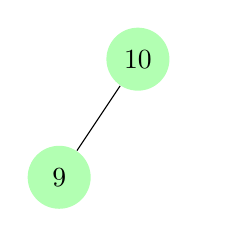
\begin{tikzpicture}[level distance=15mm, sibling distance=20mm]
        \tikzstyle{every node}=[fill=green!30,circle,inner sep=1pt, minimum size=8mm]
        \tikzstyle{level 1}=[sibling distance=20mm, set style={{every node}+=[fill=green!30]}]
        \tikzstyle{level 2}=[sibling distance=15mm, set style={{every node}+=[fill=green!30]}]
        \tikzstyle{level 3}=[sibling distance=10mm, set style={{every node}+=[fill=green!30]}]
        \tikzstyle{level 4}=[sibling distance=10mm, set style={{every node}+=[fill=green!30]}]

% This figure represents the BST after step 2. 

        \node {10} child {node {9} } child[fill=none] {edge from parent[draw=none]};

    \end{tikzpicture}
    \caption{Step 2}
\end{minipage}
\vspace{1cm}

\begin{minipage}{0.8\textwidth}
    \centering
    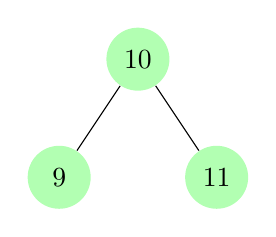
\begin{tikzpicture}[level distance=15mm, sibling distance=20mm]
        \tikzstyle{every node}=[fill=green!30,circle,inner sep=1pt, minimum size=8mm]
        \tikzstyle{level 1}=[sibling distance=20mm, set style={{every node}+=[fill=green!30]}]
        \tikzstyle{level 2}=[sibling distance=15mm, set style={{every node}+=[fill=green!30]}]
        \tikzstyle{level 3}=[sibling distance=10mm, set style={{every node}+=[fill=green!30]}]
        \tikzstyle{level 4}=[sibling distance=10mm, set style={{every node}+=[fill=green!30]}]

% This figure represents the BST after step 3. 

        \node {10} child {node {9} } child {node {11} };

    \end{tikzpicture}
    \caption{Step 3}
\end{minipage}
\vspace{1cm}

\end{figure}
\newpage

\begin{figure}[h!]
\centering

\begin{minipage}{0.8\textwidth}
    \centering
    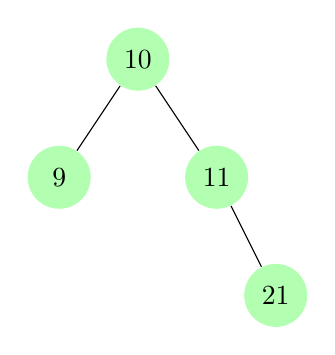
\begin{tikzpicture}[level distance=15mm, sibling distance=20mm]
        \tikzstyle{every node}=[fill=green!30,circle,inner sep=1pt, minimum size=8mm]
        \tikzstyle{level 1}=[sibling distance=20mm, set style={{every node}+=[fill=green!30]}]
        \tikzstyle{level 2}=[sibling distance=15mm, set style={{every node}+=[fill=green!30]}]
        \tikzstyle{level 3}=[sibling distance=10mm, set style={{every node}+=[fill=green!30]}]
        \tikzstyle{level 4}=[sibling distance=10mm, set style={{every node}+=[fill=green!30]}]

% This figure represents the BST after step 4. 

        \node {10} child {node {9} } child {node {11} child[fill=none] {edge from parent[draw=none]} child {node {21} }};

    \end{tikzpicture}
    \caption{Step 4}
\end{minipage}
\vspace{1cm}

\begin{minipage}{0.8\textwidth}
    \centering
    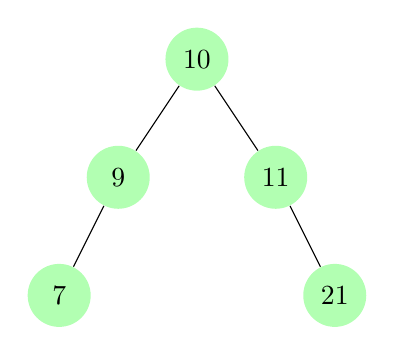
\begin{tikzpicture}[level distance=15mm, sibling distance=20mm]
        \tikzstyle{every node}=[fill=green!30,circle,inner sep=1pt, minimum size=8mm]
        \tikzstyle{level 1}=[sibling distance=20mm, set style={{every node}+=[fill=green!30]}]
        \tikzstyle{level 2}=[sibling distance=15mm, set style={{every node}+=[fill=green!30]}]
        \tikzstyle{level 3}=[sibling distance=10mm, set style={{every node}+=[fill=green!30]}]
        \tikzstyle{level 4}=[sibling distance=10mm, set style={{every node}+=[fill=green!30]}]

% This figure represents the BST after step 5. 

        \node {10} child {node {9} child {node {7} } child[fill=none] {edge from parent[draw=none]}} child {node {11} child[fill=none] {edge from parent[draw=none]} child {node {21} }};

    \end{tikzpicture}
    \caption{Step 5}
\end{minipage}
\vspace{1cm}

\end{figure}
\newpage

\end{document}
